\label{ch5}
\section{簡介}
在前一章節,利用專注式機制學習較好的向量表示,成功將平均準確率大幅提升,然而產生的查詢詞向量跟語音文件向量,就算為相似發音的詞,如hand跟hands,他們的向量表示卻大不相同。在本章中,想引入語音詞向量(Audio
Word2vec)的概念,能夠使模型學到詞的相關性,且語音詞向量是非監督式的學習方法,跟動態時間規劃的方法一樣,想嘗試以非監督式的方法,也能夠有進步。在語音詞向量模型中,會有每段詞的語音序列,才能夠訓練並產生出語音詞向量。但是我們在語音文件的部分,並無法得知每個詞的段落,所以本章想嘗試將即使不切出一段詞的語音序列而是將整段語音文件去產生出語音詞向量,並藉由分類器依據查詢詞的語音詞向量跟語音文件的語音詞向量判斷語音文件是否出現查詢詞。

\section{語音詞向量}
語音詞向量的概念為詞向量(Word Vector)的延伸,詞向量又稱詞嵌入(Word
Embedding)能夠將詞轉成有意義的向量。原本詞的表示方法常用的為是1-of-N編
碼(1-of-N
Encoding),也就是產生一個維度$N$的向量,$N$為辭典的詞數目,每一維度對應到一個詞,一個詞向量只有在該詞所對應到的維度其值為$1$,其$N-1$個維度的值都是$0$。此種表示法有其缺點,首先,$N$的維度都在數萬至數十萬的量級,導致詞向量的維度非常大。再者,此種表示法將所有的詞是為獨立,即便為兩個同義詞(Synonym),他們的1-of-N編碼之間也毫無關聯。而詞嵌入表示能夠產生分佈式表示(Distributed
Representation),將詞由原本的$N$維降低為幾百維度,且每一維度不在只有$1$或$0$,而是一連續的實數。且將語意關係或句法結構的關係,用兩個向量之間的歐式距離(Euclidean
Distance)或餘弦相似度(Cosine
Similarity)之大小就能呈現出來,例如母親與父親的歐式距離跟國王與皇后的歐式距離是相差不遠的。
語音詞向量則是希望在給定語音輸入下,也能夠產生固定維度的分佈式表示。
\begin{figure}[h]
\centering
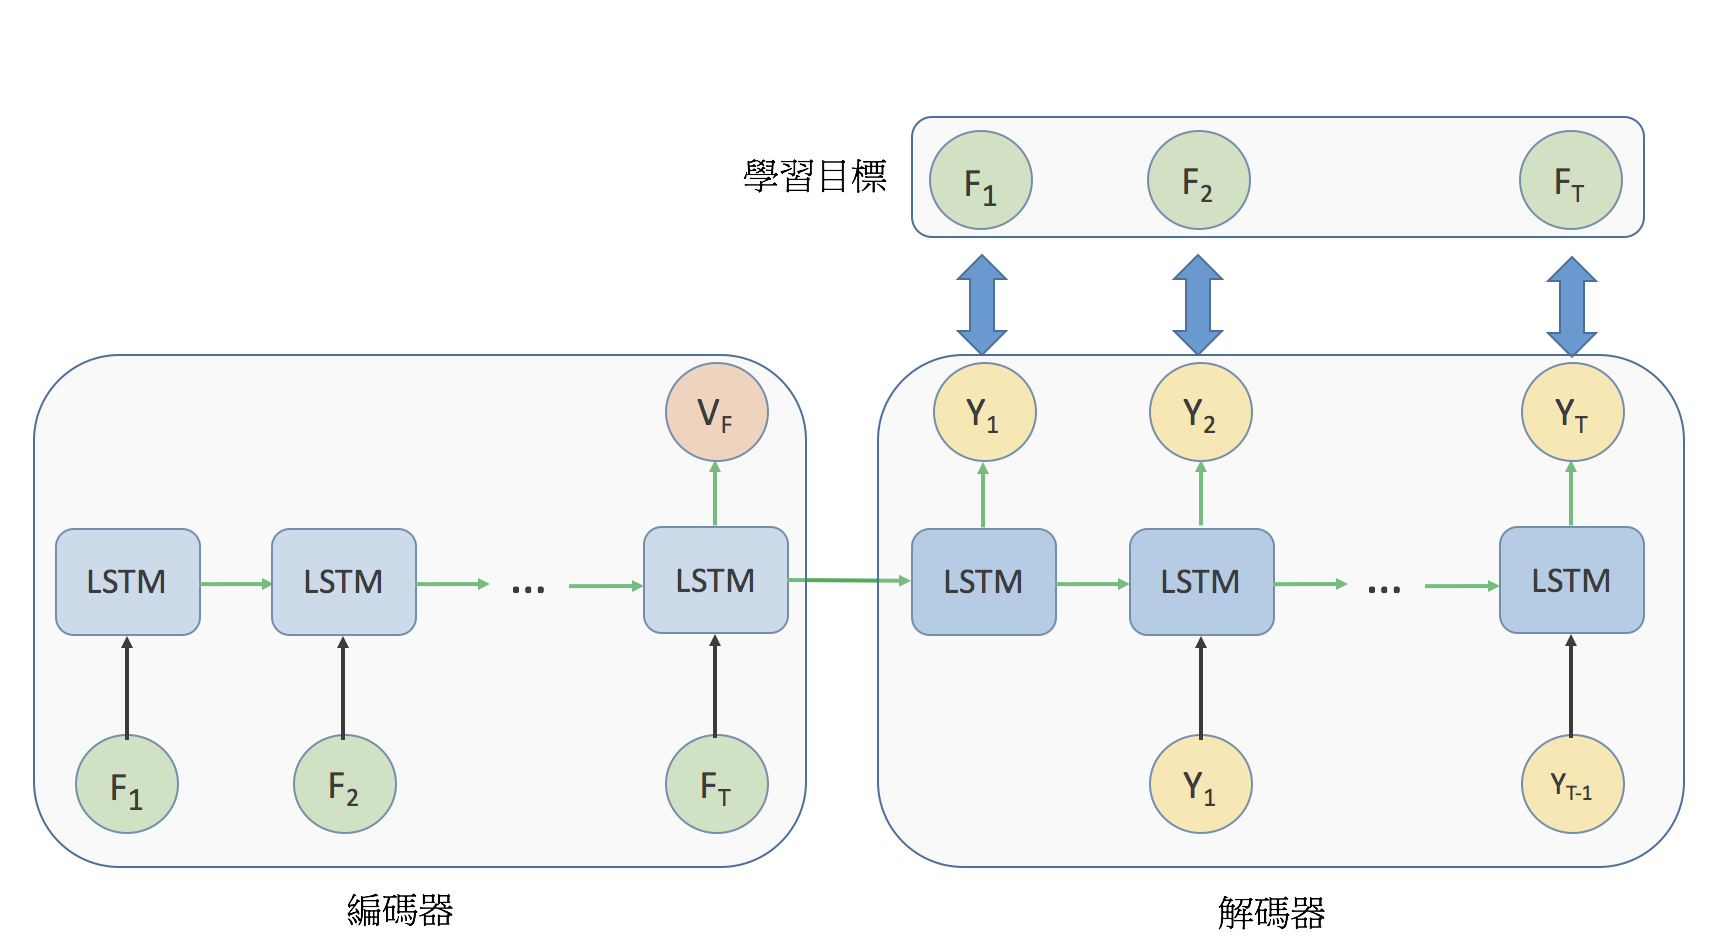
\includegraphics[scale=0.5]{images/ch5_seq2seq.png} 
\caption{語音詞向量模型圖}
\label{ch5_seq2seq}
\end{figure}
\label{ch5_seq2seq}

圖\ref{ch5_seq2seq}為語音詞向量的模型架構,基本概念仍為先前在\ref{seq2seq}章中提到的序列對序列的架構。編碼器會先將語音序列依據每個時間點$F_t$一一當作輸入,在看完整段序列後,產生一個維度固定的隱藏狀態。接著解碼器會將隱藏狀態當作初始狀態,一一產生出每個時間點的輸出$Y_t$。使其$Y_t$跟學習目標$F_t$要能夠完全相同,模型會嘗試降低$Y_t$跟$F_t$的方均根差(Root-Mean-Square
Error)。最後取其隱藏狀態當作語音序列的分佈式向量表示,即為語音詞向量。
\section{模型架構}
\subsection{模型簡介}
模型架構如圖\ref{ch5_seq2seq},編碼器將輸入的語音序列一一讀過產生出隱藏狀態,編碼器藉由隱藏狀態還原成原本的語音序列。唯一和語音詞向量不同的部分,訓練語音詞向量的資料為單個字語音序列,而此章的訓練資料並非單個字的語音序列,而是整個語音文件的序列。
\subsection{推理機制(Inference mechanism)}
在完成語音詞向量的訓練後,模型能夠藉由推理機制得到一個分數,利用此分數判別查詢詞出現在語音文件的機率。圖\ref{ch5_model}為本章推理機制示意圖,遞迴類神經網路編碼器會將查詢詞序列$Q_1,Q_2,...Q_T$編碼產生$V_Q$,語音文件序列$D_1,D_2,...,D_N$編碼產生$V_D$。接著,遞迴類神經網路解碼器會將$V_Q$跟$V_D$還原成原本的語音序列$\hat{Q_1},\hat{Q_2},...\hat{Q_T}$、$\hat{D_1},\hat{D_2},...,\hat{D_N}$,希望使其跟原本的序列越相近。最後,依照查詢詞向量$V_Q$跟語音文件向量$V_D$的歐式距離的分數排序,計算出平均準確率。

圖\ref{ch5_model}上有分別畫出語音文件跟查詢詞的編碼器,但是編碼器為同一組的遞迴類神經網路,負責將語音文件跟查詢詞編碼成向量。
\begin{figure}
\centering
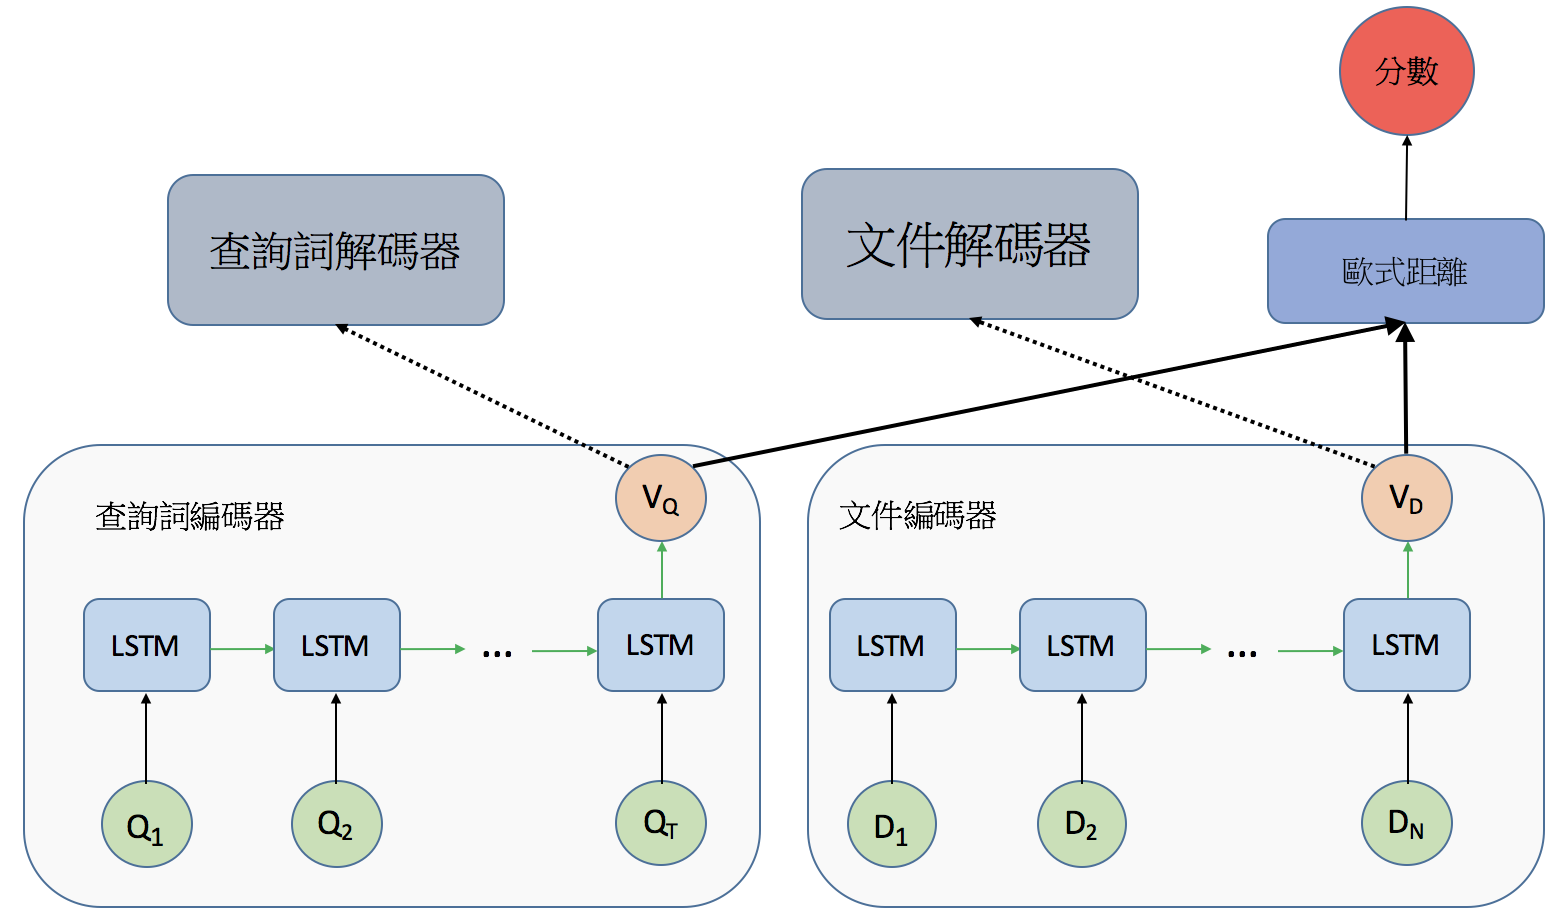
\includegraphics[scale=0.5]{images/ch5_model.png} 
\caption{模型推論機制示意圖}
\label{ch5_model}
\end{figure}
\subsection{訓練方式}
此時因模型需要能夠還原成原本的語音序列,其損失函數為均方根差如式\ref{eq:ch5_RMSE},使其編碼向量經過解碼器後的輸出跟其原始語音序列越相近。
\begin{equation}
\label{eq:ch5_RMSE}
L_{rmse} (\bold{x},\bold{y}) = \sum_{i=1}^{T}
RMSE(\bold{x}_i-\bold{y}_i) = \sum_{i=1}^{T} \sum_{j=1}^D \sqrt{(x_{ij}-y_{ij})^2}
\end{equation}
其中RMSE為方均根差,$\bold{x}$為輸入之語音序列,$\bold{y}$為模型還原之語音序列,$\bold{x}_i$為時間點$i$之聲學特徵,$\bold{y}_i$
為時間點$i$之模型還原聲學特徵,T為輸入序列長度,D為聲學特徵向量維度。最佳化演算法採用Adam演算法,採用二次正規化並給予權重0.001。

\section{實驗與分析}
\subsection{實驗設定與基準實驗}
\begin{itemize}
\item{實驗設定}

訓練語料為LIBRISPEECH 的英語語料,從train-clean-360
取出500種查詢詞,30,000個語音文件當作訓練語料。測試語料跟章節\ref{ch4}的設定相同,分成測試集$1$(查詢詞聲學特徵跟訓練語料相同)、測試集$2$(查詢詞聲學特徵跟訓練集不同)、測試集$3$(查詢詞未出現在訓練集)。
\item{基準實驗}

基準實驗仍為利用動態時間規劃得到的分數,在分別在測試集$1$得到0.6173的平均準確率,測試集$2$得到0.5778的平均準確率,測試集$3$得到0.5668的平均準確率。
\end{itemize}
\subsection{實驗結果與分析}

\begin{table}[h]
	 \centering
	 \caption{語音詞向量之實驗結果}
	 \label{table:ch5_a2v}
	 \begin{tabular}{|c|c|c|c|}
		 \hline
		 模型架構 & 測試集1 & 測試集2 & 測試集3 \\
		 \hline
		 基準實驗 & 0.6173 & 0.5778 & 0.5678\\
		 \hline
		 一層長短期記憶網路& 0.6040 & 0.5890 & 0.5793 \\
		 \hline
		 兩層長短期記憶網路& 0.6160 &0.6038 &0.5988\\
		 \hline
		 三層長短期記憶網路& {\color{red}0.6223} &0.6127 &0.6011\\
		 \hline
	   \end{tabular}
\end{table}
表\ref{table:ch5_a2v}為實驗之結果,在此章比較了不同層數的長短期記憶網路,而每層的記憶網路細胞個數為$128$個。從表中可以看出,利用語音詞向量的結果跟基準實驗差異不大,只有在層數較深的模型下,才略贏基準實驗。

動態時間規劃跟語音詞向量皆為非監督式的學習方法,所以都不需要利用到標記的資料,然而語音詞向量仍須有訓練語料才能夠學習,這是語音詞向量的劣勢。且本章並未將語音文件切成文字片段在進行訓練,而是以整段語音文件進行訓練,這表示產生出來的向量代表了整個語音文件,並不是表示單一個詞,而計算語音查詢詞跟語音文件之間的歐式距離,若語音文件出現跟查詢詞相似的詞但未出現查詢詞,此時利用歐式距離判別會產生出偏差,為此方法的一大缺失。但語音詞向量在此表現卻能跟基準實驗抗衡,是蠻意外的。
\begin{figure}[h]
\centering
\subfloat[]{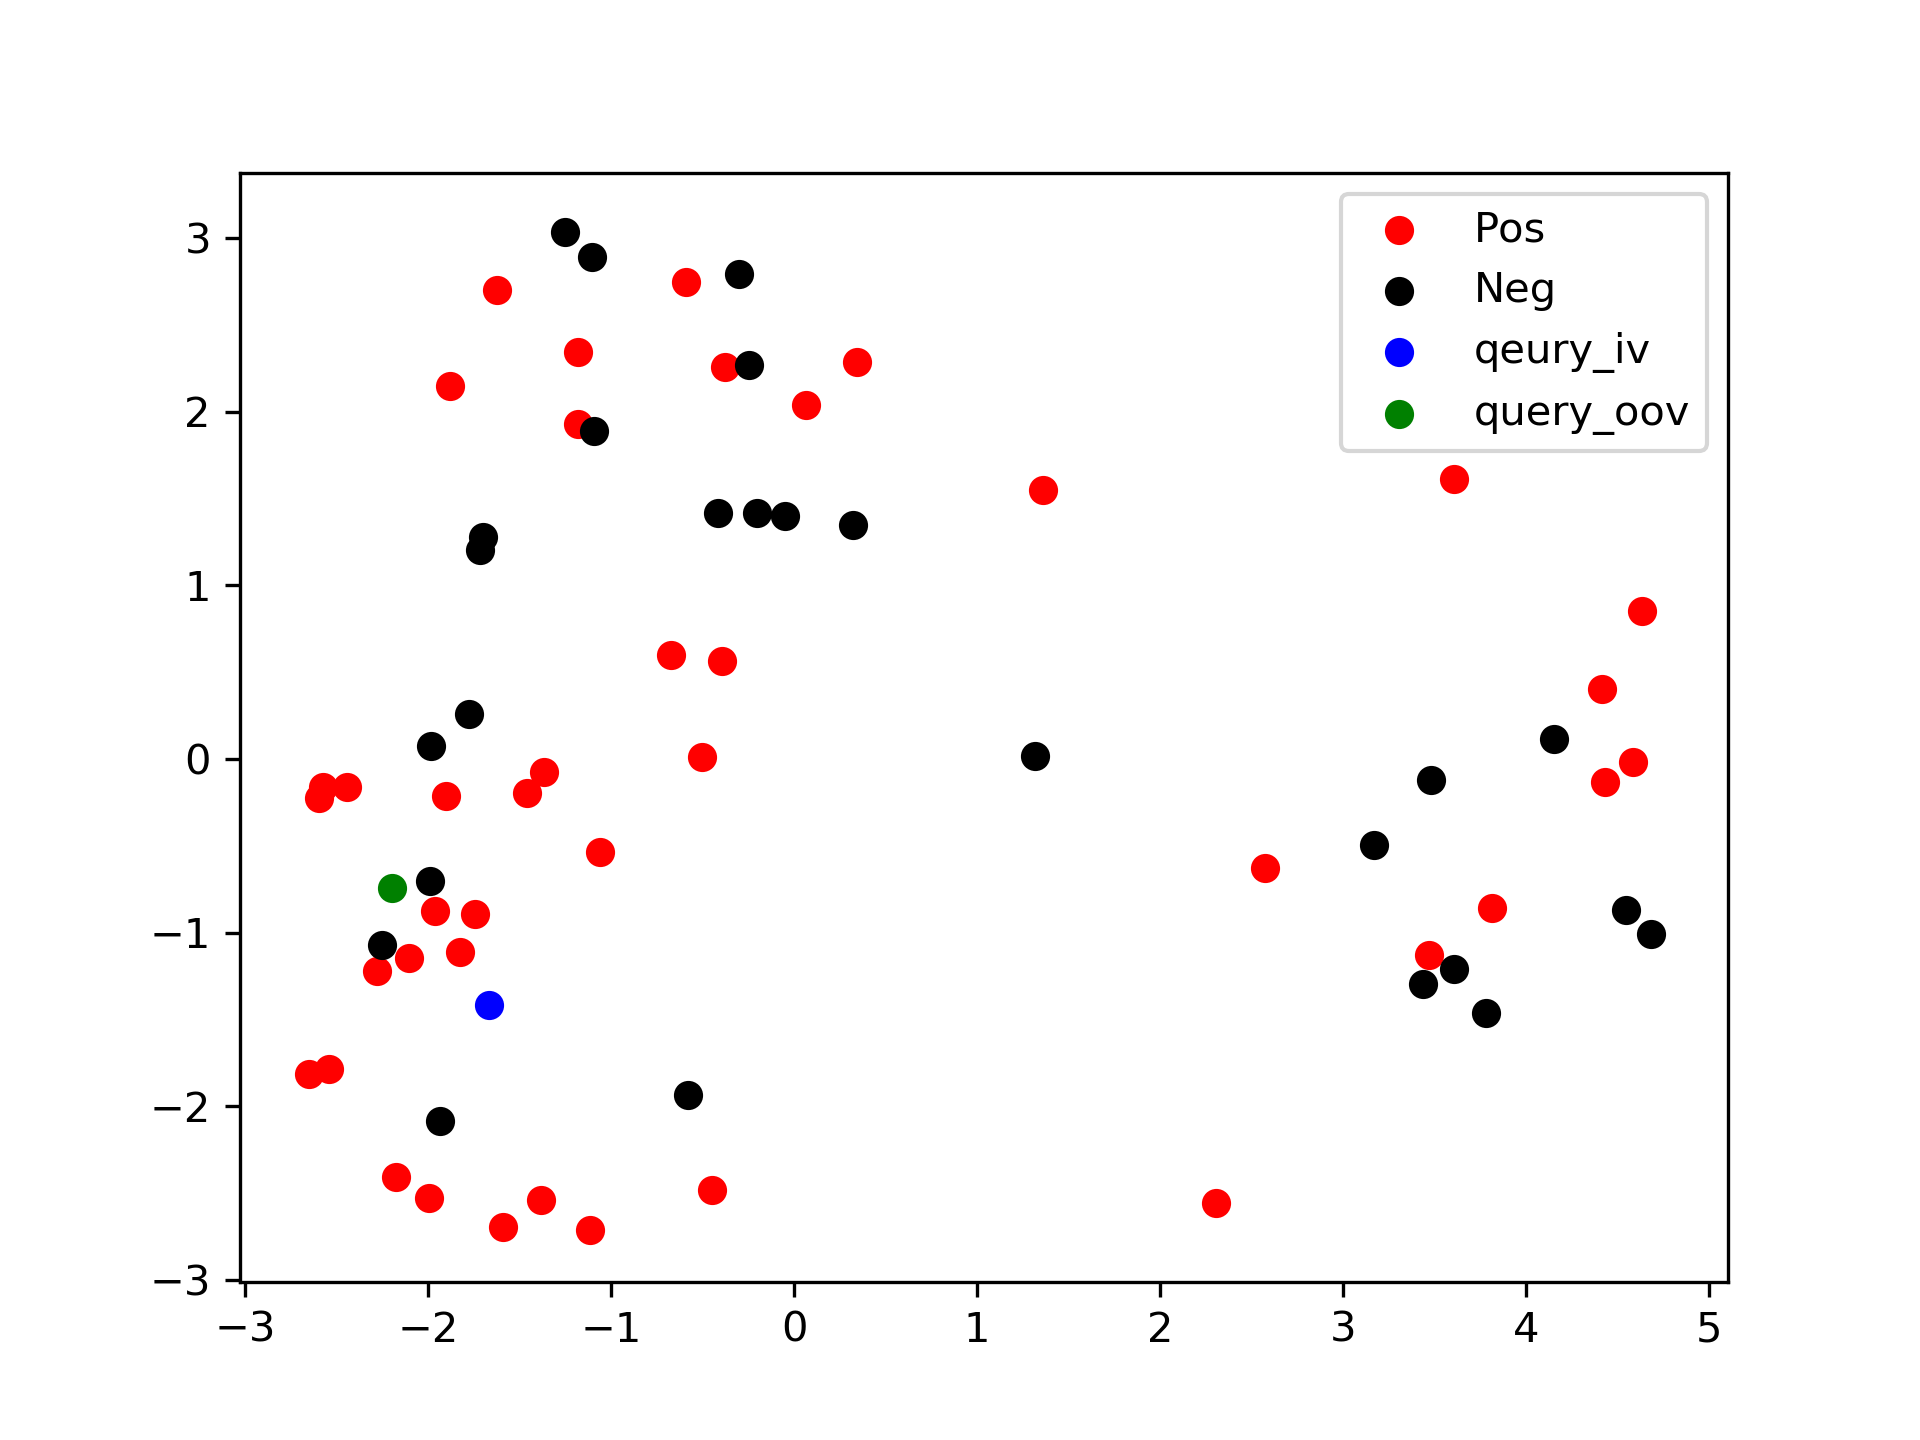
\includegraphics[scale=0.4]{images/ch5_pca1.png}}
\\
\subfloat[]{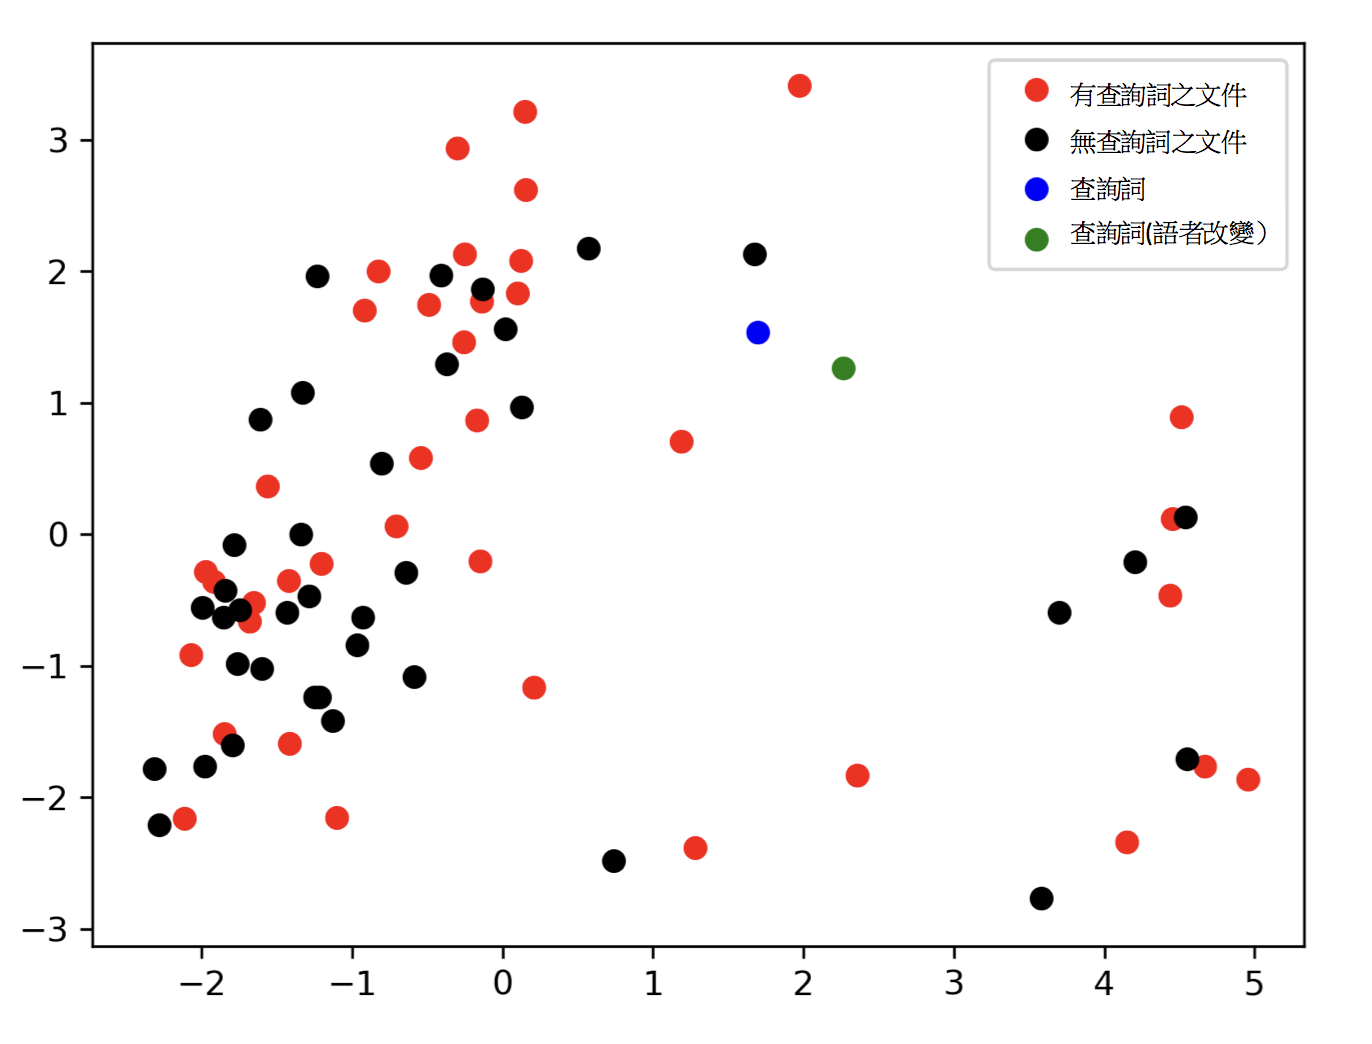
\includegraphics[scale=0.4]{images/ch5_pca2.png}}
\\
\caption{語音詞向量視覺圖}
\label{fig:ch5_vis}
\end{figure}

圖\ref{fig:ch5_vis} 為將查詢詞跟文件的語音詞向量,藉由主成份分析(Principal
Components
Analysis)\cite{dunteman1989principal}將高維的語音詞向量降成兩維,所畫出的圖。圖上紅點代表查詢詞出現的文件(Postive),黑點代表未出現查詢詞之文件(Negative),藍點為出現在訓練集的查詢詞聲學訊號,綠點為未出現在訓練集的查詢詞聲音訊號。
可以從圖上明顯地看出,依文件跟查詢詞的歐式距離作為判定不太可行的,語音文件的向量包含的是整個文件的資訊,跟查詢詞的向量是有極大差異的。但可以看出兩張圖中,不同聲學特徵的查詢詞兩者的歐式距離是近的,代表語音詞向量仍有學習到相同查詢詞的特性。圖\ref{ch5_query_vis}將查詢詞的語音詞向量透過主成份分析畫成的二維圖,可以看出DRIPPING跟JOINING為一群,PRECAUTION跟AVERSION也很相近。雖然查詢詞的訓練資料很少,但語音詞向量仍有抓到其查詢詞的特性。

\begin{figure}[h]
\centering
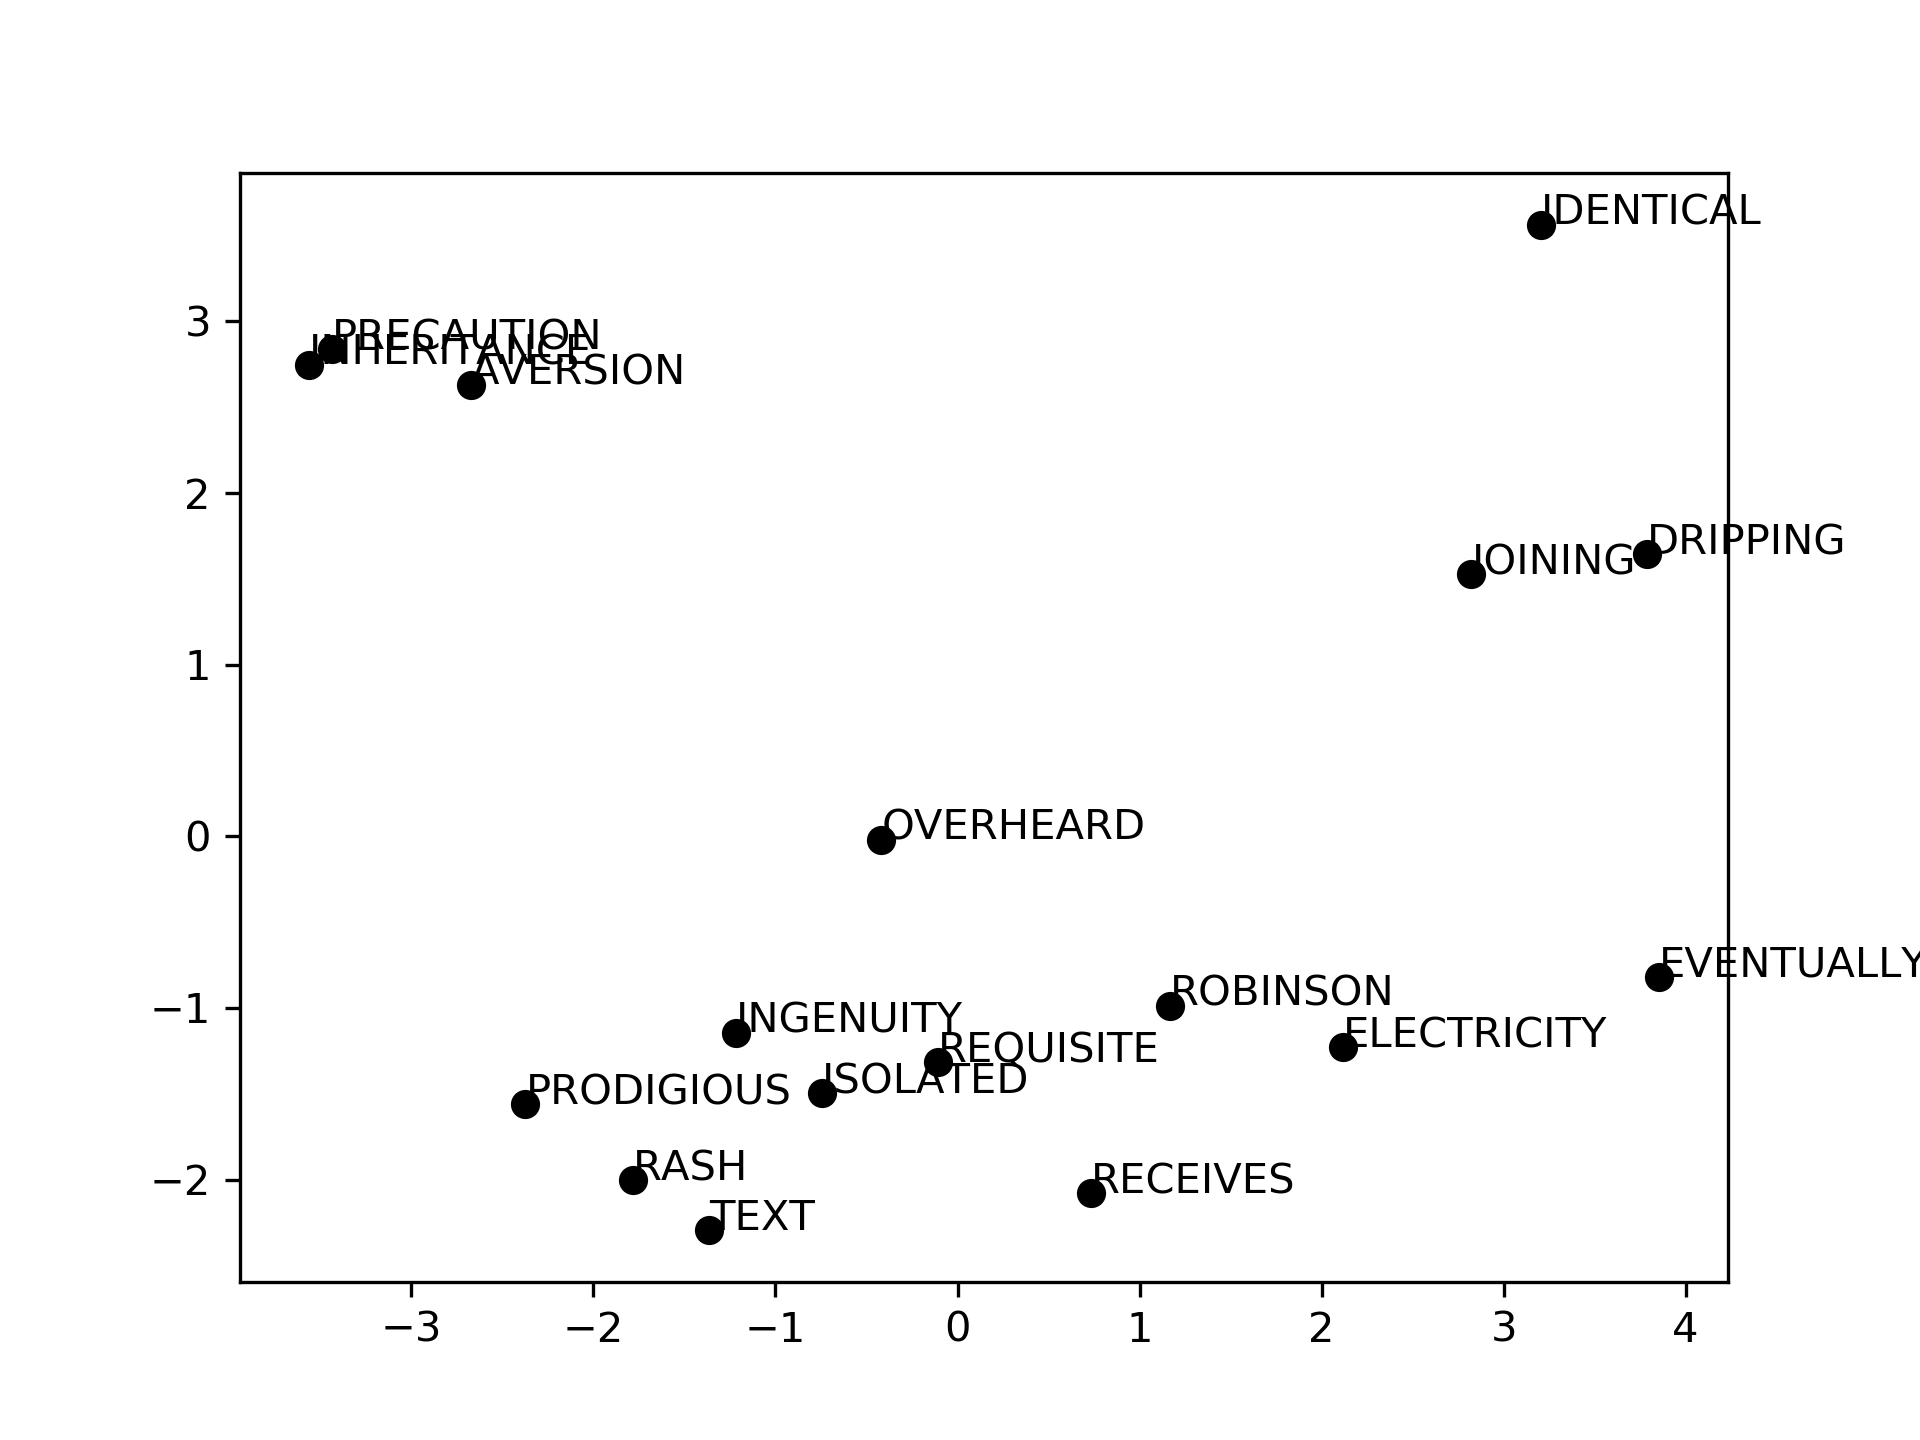
\includegraphics[scale=0.7]{images/ch5_query_vis.png} 
\caption{查詢詞之語音詞向量視覺圖}
\label{ch5_query_vis}
\end{figure}
\vspace{10cm}
\section{本章總結}
此章中利用了語音詞向量的概念,將未切段的語音文件直接進行訓練語音詞向量的模型。將語音文件與語音查詢詞分別產生其語音詞向量,利用它們之歐式距離來判定是否出現查詢詞。語音詞向量為非監督式學習,跟基準實驗動態時間規劃相同,也能夠產生與基準實驗相抗衡的表現。將語音詞向量視覺化後,證明利用整段文件去訓練語音詞向量,產生出來的向量跟查詢詞的歐式距離並無相關性。
